\documentclass[a4paper,10pt]{article}
\usepackage{My_math_package}

\title{MATH602 - Homological algebra}
\author{Haoran Li}
\date{2020 Spring}

\makeindex[columns=2, title=Index, intoc] % Create the index

\begin{document}\sloppy % Reduce overlong words

% Maketitle
\begin{titlepage}
\begin{center}
\vspace*{1cm}
\Huge
\textbf{MATH602 - Homological algebra} \\
\vspace{2cm}
\begin{center}
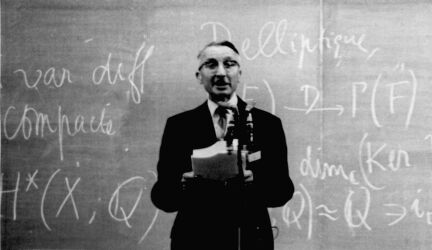
\includegraphics{Pictures/Henri_Cartan.png}
\end{center}
\vspace{2cm}
\normalsize
Taught by \texttt{Patrick Bronsnan} \\
Notes taken by \texttt{Haoran Li} \\
2020 Spring \\
\vspace{2cm}
Department of Mathematics\\
University of Maryland\\
\end{center}
\end{titlepage}

% Contents
\tableofcontents
\newpage

\section{Review of category theory}
\subfile{Category_theory/Category_theory-main.tex}
\newpage

\section{Chain complexes}
\subfile{Chain_complexes/Chain_complexes-main.tex}
\newpage

\section{Spectral sequence}
\subfile{Spectral_sequence/Spectral_sequence-main.tex}
\newpage

\section{Homeworks}
\subfile{Homeworks/Homeworks-main.tex}
\newpage

\begin{thebibliography}{}

\bibitem{An introduction to homological algebra - Weibel} 
\textit{An introduction to homological algebra} - Charles Weibel

\end{thebibliography}

\printindex
\newpage

\end{document}